\vspace{-3em}

\section*{\centering Reproducibility Summary}

% \textit{Template and style guide to \href{https://paperswithcode.com/rc2020}{ML Reproducibility Challenge 2020}. The following section of Reproducibility Summary is \textbf{mandatory}. This summary \textbf{must fit} in the first page, no exception will be allowed. When submitting your report in OpenReview, copy the entire summary and paste it in the abstract input field, where the sections must be separated with a blank line.
% }

\subsection*{Scope of Reproducibility}
% State the main claim(s) of the original paper you are trying to reproduce (typically the main claim(s) of the paper).
% This is meant to place the work in context, and to tell a reader the objective of the reproduction.
The authors claim to introduce a model for recovering the latent representation of observed data, that outperforms the state-of-the-art method for this task; namely the iVAE model. They claim that iFlow outperforms iVAE both in preservation of the original geometry of source manifold and correlation per dimension of the latent space.
%Some additional experiments examining a better baseline as well as data set difficulty are conducted.

\subsection*{Methodology}
% Briefly describe what you did and which resources you used. For example, did you use author's code? Did you re-implement parts of the pipeline? You can also use this space to list the hardware used, and the total budget (e.g. GPU hours) for the experiments.
% To reproduce the results of the paper, we aimed to reproduce the results that were reported for the iFlow model, as well as the results of the iVAE model that was used for comparison. In addition, we recreated the figures shown in the paper.
To reproduce the results of the paper, the main experiments are reproduced and the figures are recreated.
To do so, we largely worked with code from the repository belonging to the original paper. We added plotting functionality as well as various bug fixes and optimisations. Additionally, attempts were made to improve the iVAE by making it more complex and fixing a mistake in its implementation.We also tried to investigate possible correlation between the structure of the dataset and the performance. All code used is publicly available at \url{https://github.com/HiddeLekanne/Reproducibility-Challenge-iFlow}.

\subsection*{Results}
% Start with your overall conclusion --- where did your results reproduce the original paper, and where did your results differ? Be specific and use precise language, e.g. "we reproduced the accuracy to within 1\% of reported value, which supports the paper's conclusion that it outperforms the baselines". Getting exactly the same number is in most cases infeasible, so you'll need to use your judgement to decide if your results support the original claim of the paper.
The obtained mean and standard deviation of the MCC over 100 seeds are within 1 percent of the results reported in the paper.
The iFlow model obtained a mean MCC score of 0.718 (0.067). Efforts to improve and correct the baseline increased the mean MCC score from 0.483 (0.059) to 0.556 (0.061). The performance, however, remains worse than the performance of iFlow, further supporting the authors' claim that the iFlow implementation is correct and more effective than iVAE.

\subsection*{What was easy}
% Describe which parts of your reproduction study were easy. For example, was it easy to run the author's code, or easy to re-implement their method based on the description in the paper? The goal of this section is to summarize to a reader which parts of the original paper they could easily apply to their problem.
The GitHub repository associated with the paper provided most necessary code and ran with only minor changes. The code included all model implementations and data generation.
The script that was used to obtain results was provided, which allowed us to determine which exact hyperparameters were used with experiments on the iFlow models. Overall, the code was well organised and the structure was easy to follow.

\subsection*{What was difficult}
% Describe which parts of your reproduction study were difficult or took much more time than you expected. Perhaps the data was not available and you couldn't verify some experiments, or the author's code was broken and had to be debugged first. Or, perhaps some experiments just take too much time/resources to run and you couldn't verify them. The purpose of this section is to indicate to the reader which parts of the original paper are either difficult to re-use, or require a significant amount of work and resources to verify.
The specific versions of the Python libraries used were unknown, which made it infeasible to achieve the exact results from the paper when running on the same seeds.
The code used to create figures 1-3 in the original paper was missing and had to be recreated. Furthermore, the long time the models needed to train made experimentation with e.g., different hyperparameters challenging. Finally, the code was largely undocumented.

\subsection*{Communication with original authors}
% Briefly describe how much contact you had with the original authors (if any).
Communication with the authors was attempted but could not be established.

\newpage
% \textit{\textbf{The following section formatting is \textbf{optional}, you can also define sections as you deem fit.
% \\
% Focus on what future researchers or practitioners would find useful for reproducing or building upon the paper you choose.}}
\section{Introduction}
%============================ DESCRIPTION ================================
% A few sentences placing the work in high-level context. Limit it to a few paragraphs at most; your report is on reproducing a piece of work, you don’t have to motivate that work.
%============================ CONTENT ================================

Nowadays, different types of deep generative models excel at generating new data by either explicitly or implicitly modelling the distribution of the training data. However, sometimes it is useful to recover the distribution that generated the observed data, i.e. the latent distribution, rather than the data distribution itself.  It is easy to see that this is a more difficult task due to the unknown relation between the unobserved latent variables and the observed data. The concept of recovering the true latent distribution underlying the data is a form of \textit{identifiability}.

Some research has been done in this area. Previously, models (notably $\beta$-VAE \cite{burgess2018understanding} and its variations) were created with the purpose of creating \textit{disentangled} representations, where single latent units correspond to single generative factors. While related to identifiability, such models do not provide any proof or guarantee that they can recover the true latent representations.

More recently, an identifiable variation of the VAE called iVAE was proposed \cite{khemakhem2020variational}, which uses a factorised prior conditioned on an auxiliary variable to guarantee a basic form of identifiability. In practice however, the fact that this model optimises a lower bound on the posterior, rather than the actual posterior, could negatively affect the capability of the model to recover the true latent variables.

The paper "Identifying through flows for recovering latent representations" proposes \textit{iFlow}, a model that aims to alleviate these problems by using Normalising Flow models rather than VAEs \cite{li2019identifying}. The fact that Normalising flows model exact distributions rather than approximating the posterior could make them more suitable for this task.

\section{Scope of reproducibility}
\label{sec:claims}
%============================ DESCRIPTION ================================
% Introduce the specific setting or problem addressed in this work, and list the main claims from the original paper. Think of this as writing out the main contributions of the original paper. Each claim should be relatively concise; some papers may not clearly list their claims, and one must formulate them in terms of the presented experiments. (For those familiar, these claims are roughly the scientific hypotheses evaluated in the original work.)

% A claim should be something that can be supported or rejected by your data. An example is, ``Finetuning pretrained BERT on dataset X will have higher accuracy than an LSTM trained with GloVe embeddings.''
% This is concise, and is something that can be supported by experiments.
% An example of a claim that is too vague, which can't be supported by experiments, is ``Contextual embedding models have shown strong performance on a number of tasks. We will run experiments evaluating two types of contextual embedding models on datasets X, Y, and Z."

% This section roughly tells a reader what to expect in the rest of the report. Clearly itemize the claims you are testing:
% \begin{itemize}
%     \item Claim 1
%     \item Claim 2
%     \item Claim 3
% \end{itemize}

% Each experiment in Section~\ref{sec:results} will support (at least) one of these claims, so a reader of your report should be able to separately understand the \emph{claims} and the \emph{evidence} that supports them.

%\jdcomment{To organisers: I asked my students to connect the main claims and the experiments that supported them. For example, in this list above they could have ``Claim 1, which is supported by Experiment 1 in Figure 1.'' The benefit was that this caused the students to think about what their experiments were showing (as opposed to blindly rerunning each experiment and not considering how it fit into the overall story), but honestly it seemed hard for the students to understand what I was asking for.}
%============================ CONTENT ==================================

In this review, the work of the proposed iFlow model by Li et al. \cite{li2019identifying} is reproduced and examined. The aim is to reproduce the results obtained by the authors and to investigate the claims made in the paper. The claims made can be seen below. Each claim will be examined in a corresponding subsection in section \ref{sec:results}.

\begin{enumerate}
    \item Simulations on synthetic data validate the correctness and effectiveness of the proposed iFlow method and demonstrate its practical advantages over other existing methods.
    \item iFlow outperforms iVAE in identifying the original sources while preserving the original geometry of source manifold.
    \item iFlow exhibits much stronger correlation than iVAE does in each single dimension of the latent space.
    \item Making iVAE more expressive does not help it approximate the real latent space further, justifying the discrepancy in parameters.
\end{enumerate}

\section{Methodology}
\label{sec:methodology}
%============================ DESCRIPTION ================================
%Explain your approach - did you use the author's code, or did you aim to re-implement the approach from the description in the paper? Summarize the resources (code, documentation, GPUs) that you used.
%============================ CONTENT  ================================
Most of the original source code was available and used to test the reproducibility of the paper which can be found in the corresponding GitHub repository \footnote{\url{https://github.com/MathsXDC/iFlow}}. This repository itself contained code from the repository of the iVAE model\footnote{\url{https://github.com/siamakz/iVAE}} and \textit{nflows} \footnote{\url{https://github.com/bayesiains/nflows}}.

The iFlow implementations were used largely as is, while the iVAE implementation was refactored to apply modifications more easily. The \textit{nflows} code base has been removed from the repository and imported as a library instead. Furthermore, some small optimisations were made to make certain functions more efficient by vectorising them. For reproducing the results the models were trained on a GPU (see section \ref{sec:requirements}).  The code for creating the visualisations was not included in the repository and was therefore recreated.
% A comment in the files mentioned an error in the implementation because the Softplus function was applied to $\xi$ as well as $\eta$ from the natural parameters $\mathbf{\lambda (u)}$. An alternative version of the implementation was also tested where the Softplus activation function was only exerted on $\xi$, as there are no constraints on the sign of $\eta$. \\
The implementation was made using the \texttt{PyTorch} and \texttt{NumPy} libraries with \texttt{Python 3.7.9}. \texttt{TensorBoard} was used for logging of variables during training.

\subsection{Model descriptions}
%============================ DESCRIPTION ================================
%Include a description of each model or algorithm used. Be sure to list the type of model, the number of parameters, and other relevant info (e.g. if it's pretrained).
%============================ CONTENT ================================

The paper compares two models: the proposed iFlow model and the iVAE model.

The iFlow model is a variation on the Normalising Flow model \textit{rational-quadratic neural spline flows (featuring autoregressive layers)} (RQ-NSF (AR)) \cite{durkan2019neural}, where the prior has been replaced with a factorised exponential prior distribution conditioning the latent variables $z$ on auxiliary variables $u$ to obtain identifiability up to an equivalence relation. The natural parameters of the prior are obtained through a trainable multi-layer perceptron (MLP) which takes the auxiliary variable $u$ as input. Each iFlow model contains approximately 3 million trainable parameters.

The iVAE model is implemented as an extension of vanilla VAE models \cite{kingma2013auto}, using MLPs for both the encoder and decoder. The number of layers, hidden dimensions and activation functions are hyperparameters. The encoder uses two MLPs (one for mean and variance each), while the decoder uses just one. Additionally, the prior mapping the auxiliary variables $u$ to the latent variables $z$ is also implemented as an MLP. In total, the iVAE model with standard parameters has roughly 18,000 trainable parameters.

There is a significant difference in the complexities of iFlow and iVAE, seen in the number of trainable parameters the models have. The authors argue that this is not the cause of the inferior performance of the iVAE, showing that adding more layers/increasing the hidden dimensions of the model does not increase performance. However, only a limited range of parameters were used for this, resulting in only weak evidence to support the claim that the comparison is fair.
We further investigate this claim by scaling up the complexity of iVAE through various methods, namely adding residual connections and layer normalisation in addition to changing hyperparameters.

When looking at the implementation of the iVAE model, there appears to be a difference with the theory: the mean of the prior distribution is not a function of the auxiliary variables $u$, as the theory states, but simply fixed to be 0 at all times. We aim to incorporate this change into the implementation of iVAE to see if it leads to better performance.

\subsection{Dataset}
%============================ DESCRIPTION ================================
%For each dataset include 1) relevant statistics such as the number of examples and label distributions, 2) details of train / dev / test splits, 3) an explanation of any preprocessing done, and 4) a link to download the data (if available).
%============================ CONTENT  ================================
A synthetic dataset is required in order to truly know the underlying latent distribution, which is necessary for quantitative analysis of the performance.
The authors chose to use a dataset consisting of sources of non-stationary Gaussian time-series. Such data was previously used to introduce time-contrastive learning as a means of achieving identifiable non-linear independent component analysis \cite{hyvarinen2016unsupervised} and was additionally used to assess the performance of the iVAE \cite{khemakhem2020variational}.

The latent representation (source) is created as non-stationary Gaussian time series. This data consists of $M$ segments, which are modelled as Gaussian distributions with different, randomly selected mean and variance. The means are sampled from uniform distribution $[-5,5]$, while the variances are sampled from uniform distribution $[0.5,3]$.
Each segment contains $L$ samples drawn from the corresponding distribution of segment $M$. The segment labels serve as the auxiliary variables $u$.

A 3 layer invertible MLP is used to transform the samples in a non-linear manner to obtain the observable data. The invertible MLP consists of mixing matrices with the non-linear activation function $h(x)=tanh(x)+\alpha\cdot x$. The last layer does not contain a non-linear activation function. Due to the constraints of Flow models, the dimensionality $d$ of these observed data points has to be the same as the dimensionality of the latent representation $n$. The data generator allows for the addition of noise to the data points, but this is not utilised.

In the paper, results are reported on a dataset created using $M = 40$, $L = 1000$, $n = d = 5$ and $\alpha=0.1$. For visualisations of the sources and the estimations of the models, $M = 5$, $L = 1000$, $n = d = 2$ and $\alpha=0.1$ are used. This differs from the reported $M = 40$ from the original paper where the figure indicates that the true $M = 5$.

\subsection{Hyperparameters}
%============================ DESCRIPTION ================================
% Describe how the hyperparameter values were set. If there was a hyperparameter search done, be sure to include the range of hyperparameters searched over, the method used to search (e.g. manual search, random search, Bayesian optimization, etc.), and the best hyperparameters found. Include the number of total experiments (e.g. hyperparameter trials). You can also include all results from that search (not just the best-found results).
%============================ CONTENT ================================
The authors of the original paper mention specific values for some of the hyperparameters. However, for other hyperparameters only a range is provided without a clear indication of what values were used for each evaluation.

% Data hyper params
As mentioned before, for generating the data, the parameters $M = 40$, $L = 1000$, $n = d = 5$ and $M = 5$, $L = 1000$, $n = d = 2$ were used for experiments and visualisation respectively. A factorised Gaussian distribution was used as a prior for the source distributions. The means and variances for these distributions were sampled from uniform distributions $[-5,5]$ and $[0.5,3]$ respectively. The data was transformed with an invertible MLP of depth 3 with \texttt{tanh} activation function and a slope of $0.1$.

% Both models hyperparamters
Both the iVAE and iFlow used the same batch size ($B = 64$) and learning rate of $0.001$. A learning rate drop factor of 0.25 was used and a learning patience of 10. An Adam optimiser without weight decay and with standard $\beta$ values (0.9, 0.999) and $\epsilon$ (1e-8) was used \cite{kingma2014adam}. A learning rate scheduler to reduce the learning rate with a factor 0.1 on plateaus ensured that the learning rate decreased over time.

% iFlow model
The iFlow models were initialised with a flow length of 10 with 8 bins. The Rational Quadratic Neural Spline Flows with Autoregressive transforms (RQNSF-AR) was used as flow type. The Softplus activation was exerted on the natural parameters.

% iVAE model
To replicate the iVAE baseline, a model with a hidden dimensionality of 50, a latent dimension equal to that of the data ($d = n = 5$) and 3 layer MLPs with leaky ReLU with $\alpha = 0.1$ as activation function. These same hyperparameters were used for the additional experiments.

\subsection{Experimental setup and code}
%============================ DESCRIPTION ================================
%Include a description of how the experiments were set up that's clear enough a reader could replicate the setup.
%Include a description of the specific measure used to evaluate the experiments (e.g. accuracy, precision@K, BLEU score, etc.).
%Provide a link to your code.
%============================ CONTENT ================================
The code for this reproducibility review is publicly available at \url{https://github.com/HiddeLekanne/Reproducibility-Challenge-iFlow}. As mentioned earlier, this code consist of a combination of the iFlow and iVAE codebases (see section \ref{sec:methodology}).

% Standard Experiment setup
The iFlow and iVAE models were trained with 100 different seeds to generate datasets and the aforementioned hyperparameters. As is standard for these types of models, the iFlow model was trained using negative log likelihood as a loss, and the iVAE was used using the ELBO as a loss \cite{kingma2013auto}.
Model performance was evaluated using the mean correlation coefficient (MCC) between the original source of the data and the estimated latent variables from the models.

\subsection{Computational requirements}
\label{sec:requirements}
%============================ DESCRIPTION ================================
% Include a description of the hardware used, such as the GPU or CPU the experiments were run on.
% For each model, include a measure of the average runtime (e.g. average time to predict labels for a given validation set with a particular batch size).
% For each experiment, include the total computational requirements (e.g. the total GPU hours spent).
% (Note: you'll likely have to record this as you run your experiments, so it's better to think about it ahead of time). Generally, consider the perspective of a reader who wants to use the approach described in the paper --- list what they would find useful.
%============================ CONTENT ================================
All experiments were run on the LISA system\footnote{\url{https://userinfo.surfsara.nl/systems/lisa}} provided by the University of Amsterdam. This system provides multi-core nodes for research projects. A GeForce GTX 1080 Ti was used to train the models.

Training of iVAE models for 100 different seeds took approximately 2 hours. Training of a single iFlow model with a flow length of 10 took approximately 45 minutes. To alleviate some of the computational cost, the 100 models were trained in two worker nodes instead of one. This totalled to approximately 1.5 days of training per 100 models.

Upgrading of computational resources would not garner better results, with respect to time, based on the fact that the bottleneck for the computations was the speed of a single thread CPU. Attempts were made to improve this performance but these did not decrease training time.

\section{Results}
\label{sec:results}
%============================ DESCRIPTION ================================
% Start with a high-level overview of your results. Do your results support the main claims of the original paper? Keep this section as factual and precise as possible, reserve your judgement and discussion points for the next "Discussion" section.
%============================ CONTENT ================================

In this section, results from the original paper are recreated. In addition, some further experiments were done of which the results can also be found below. These additional experiments consist of improving the existing base line proposed in the paper, as well as exploring the relation between the complexity of the synthetic data and the achieved MCC scores.

\begin{figure}[ht]
  \begin{subfigure}[b]{0.5\textwidth}
    \centering
    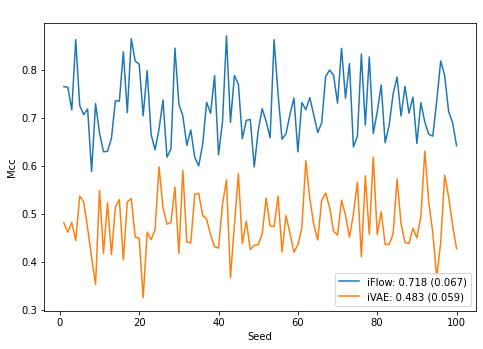
\includegraphics[width=\textwidth]{Reproducibility_Challenge_2020/IMG/scores/Mcc_Score.png}
    \caption{}
    \label{fig:MCCscores:a}
  \end{subfigure}%%
  \begin{subfigure}[b]{0.5\textwidth}
    \centering
    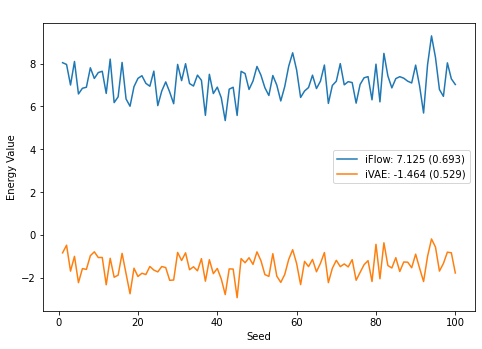
\includegraphics[width=\textwidth]{Reproducibility_Challenge_2020/IMG/scores/Log_Likelihood.png}
    \caption{}
    \label{fig:MCCscores:b}
  \end{subfigure}
  \caption{Comparison of identifying performance (MCC) and the energy value (log-likelihood) versus seed number respectively.}
  \label{fig:MCCscores}
\end{figure}

\subsection{Results reproducing original paper}
%============================ DESCRIPTION ================================
% For each experiment, say 1) which claim in Section~\ref{sec:claims} it supports, and 2) if it successfully reproduced the associated experiment in the original paper.
% For example, an experiment training and evaluating a model on a dataset may support a claim that that model outperforms some baseline.
% Logically group related results into sections.
%============================ CONTENT ================================

\subsubsection{Comparison of identifying performance}
The MCC scores and log-likelihood over 100 seeds are displayed in figure \ref{fig:MCCscores:a} and figure \ref{fig:MCCscores:b} respectively. The figures show that there is high variance in MCC scores for different datasets. The iFlow models obtained a mean accuracy of $0.718$ with a standard deviation of $0.067$ whereas the iVAE models obtained a mean accuracy of $0.483$ with a standard deviation of $0.059$ which is in compliance with the results produced in the original paper. The results for the iVAE models are significantly worse than in the original iVAE paper. An improvement to the implementation was made to better emulate the performance of this paper which resulted in a fairer comparison (see section \ref{sec:alt methods}).

%iFlow text: Moreover, Fig-ure 2(b) also showcases that the energy value of iFlow is much higher than that of iVAE, which serves as evidence that the optimization of the evidence lower bound, as in iVAE, would lead to sub-optimal identifiability.  As is borne out empirically, the gap between the evidence lower bound and the conditional marginal likelihood is inevitably far from being negligible in practice.

As can be seen in figure \ref{fig:MCCscores:b}, the energy values of the iVAE are significantly lower compared to those of iFlow, matching the results of the paper. The authors noted that the difference in energy values could indicate that the gap between the ELBO and the actual log likelihood is not negligible.
% The energy values in figure \ref{fig:MCCscores:b} show that the iVAE models have a significantly lower log-likelihood.
% As noted by the authors, this gap between the ELBO and the marginal likelihood is significant.
% However, these two values represent different measurements as calculations of the marginal likelihood for the iVAE model are intractable.

% \begin{figure}[ht]
%   \begin{subfigure}[b]{0.5\textwidth}
%     \centering
%     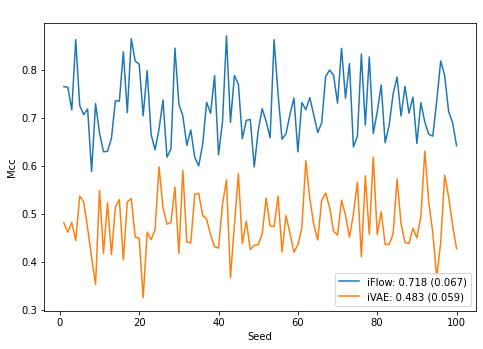
\includegraphics[width=\textwidth]{Reproducibility_Challenge_2020/IMG/scores/Mcc_Score.png}
%     \caption{}
%     \label{fig:MCCscores:a}
%   \end{subfigure}%%
%   \begin{subfigure}[b]{0.5\textwidth}
%     \centering
%     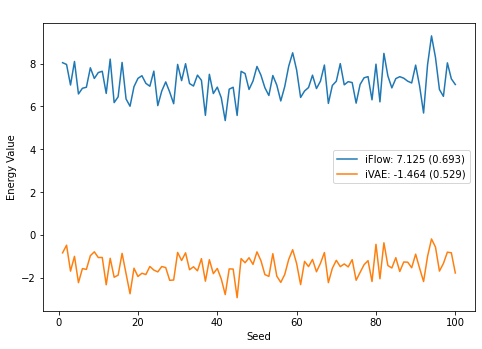
\includegraphics[width=\textwidth]{Reproducibility_Challenge_2020/IMG/scores/Log_Likelihood.png}
%     \caption{}
%     \label{fig:MCCscores:b}
%   \end{subfigure}
%   \caption{Comparison of identifying performance (MCC) and the energy value (log-likelihood) versus seed number respectively.}
%   \label{fig:MCCscores}
% \end{figure}

\subsubsection{Preservation of original source manifold geometry}
\label{sec:geometry}
% Performance of 2D latent variables
% These results examine the claim that iFlow outperforms iVAE in identifying the original sources while preserving the original geometry of source manifold.
Figure \ref{fig:2D} shows the 2D visualisation for different data seeds. The original paper stated that an $M = 40$ was used but figures indicated that this should be $M = 5$.

The results largely support the claim of the author that the original geometry of the source manifold is preserved. The estimations from the iFlow model seem more similar to the original source than the estimations from the iVAE models, although it still contain artefacts from the observations. Figure \ref{fig:2D:a} is an example of such where the latent dimensions are not successfully recovered. In other examples, the original Gaussian distributions are mostly recovered apart from some transformation as was the case in the original paper. The collapse of the latent space from iVAE models observed in the original paper was not prevalent during experiments. However, the preservation of the original geometry of the source manifold is better captured by the iFlow models.

\begin{figure}[ht]
    \centering
  \begin{subfigure}[b]{0.4\textwidth}
    \centering
    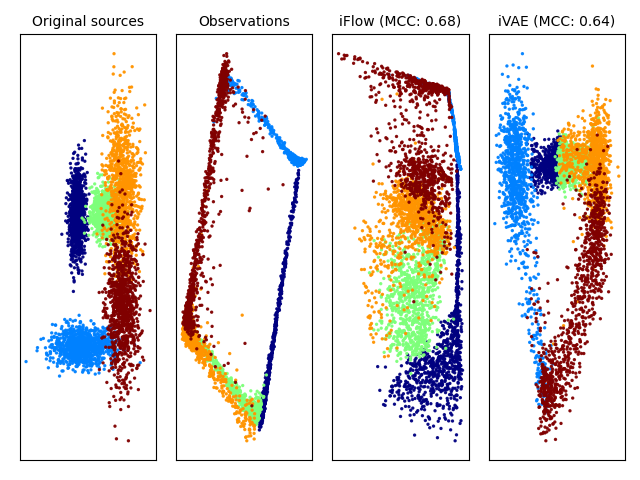
\includegraphics[width=\textwidth]{Reproducibility_Challenge_2020/IMG/2D_perf/2D_performance_old_seed21.png}
    \caption{}
    \label{fig:2D:a}
  \end{subfigure}%%
  \begin{subfigure}[b]{0.4\textwidth}
    \centering
    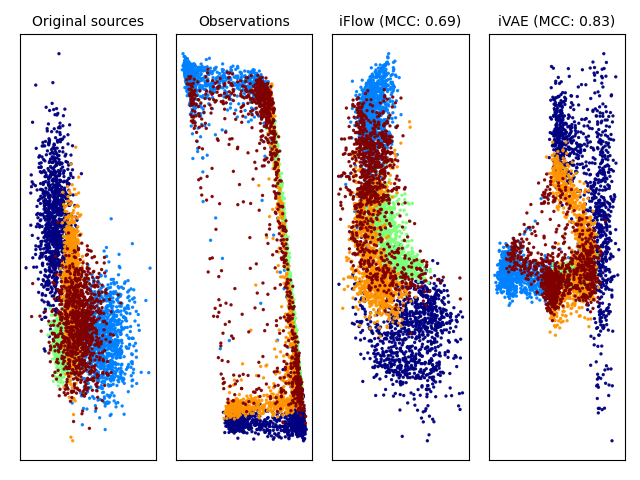
\includegraphics[width=\textwidth]{Reproducibility_Challenge_2020/IMG/2D_perf/2D_performance_old_seed42.png}
    \caption{}
    \label{fig:2D:b}
  \end{subfigure}
  \begin{subfigure}[b]{0.4\textwidth}
    \centering
    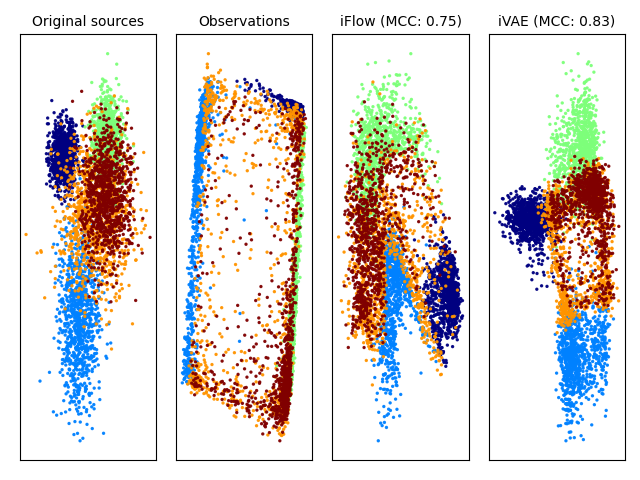
\includegraphics[width=\textwidth]{Reproducibility_Challenge_2020/IMG/2D_perf/2D_performance_old_seed66.png}
    \caption{}
    \label{fig:2D:c}
  \end{subfigure}%%
  \begin{subfigure}[b]{0.4\textwidth}
    \centering
    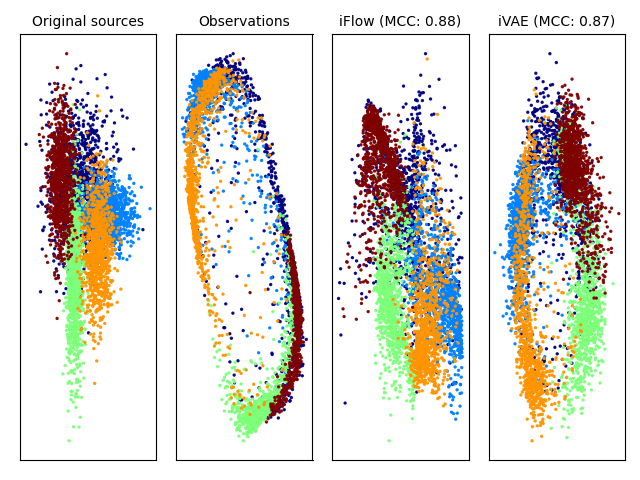
\includegraphics[width=\textwidth]{Reproducibility_Challenge_2020/IMG/2D_perf/2D_performance_old_seed77.png}
    \caption{}
    \label{fig:2D:d}
  \end{subfigure}
  \caption{Visualisation of 2D-cases}
  \label{fig:2D}
\end{figure}

\subsubsection{Separate latent dimension correlation}
\label{sec:latentcorr}
% Performance per dimension
Figure \ref{fig:latentcorr1} and figure \ref{fig:latentcorr2} show the correlation between the source signal used to generate the data and the latent variables recovered by the iFlow and iVAE models. Figure \ref{fig:latentcorr1} shows the results of the best performing iFlow, which we assume is what figure 3 of the original paper also depicts. For fairness, we also show the results for the dataset that iVAE performed best on in figure \ref{fig:latentcorr2}.

These results largely support the claim that iFlow exhibits stronger correlation than does iVAE in each single dimension of the latent space: while this is generally the case, it does occur for some datasets that iVAE has a higher correlation coefficient than iFlow on one or even two of the latent dimensions, as shown in figure \ref{fig:latentcorr2}.

\begin{figure}[!htbp]
    \centering
    \begin{minipage}[b]{\textwidth}
        \centering
       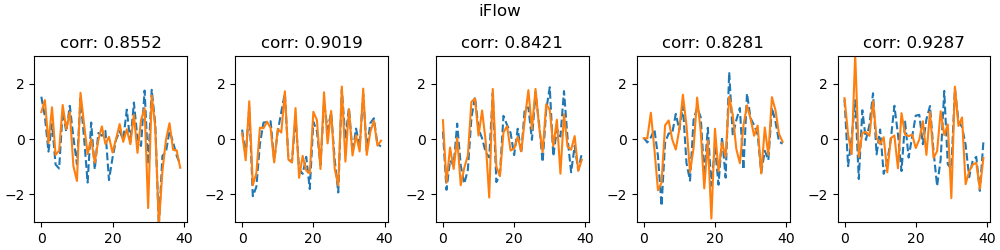
\includegraphics[width=0.8\textwidth]{Reproducibility_Challenge_2020/IMG/latent_corr/best_iFlow_42.png}
    \end{minipage}
    \begin{minipage}[b]{\textwidth}
    \centering
       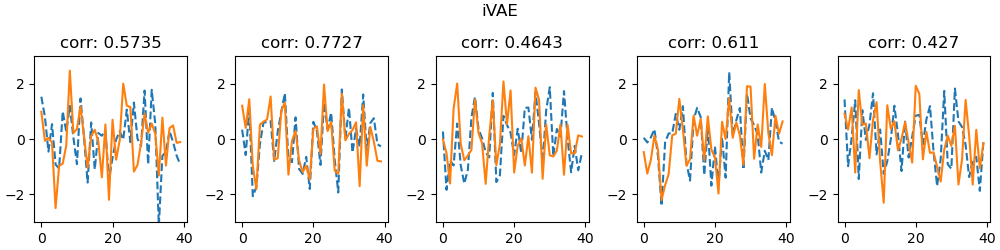
\includegraphics[width=0.8\textwidth]{Reproducibility_Challenge_2020/IMG/latent_corr/iVAE_42.png}
    \end{minipage}
    \caption{Comparison of the latent variables recovered by the models (orange lines) to the true latent variables (dashed blue lines) for individual dimensions. This figure shows results for the seed that resulted in the best iFlow performance.}
    \label{fig:latentcorr1}
\end{figure}

\begin{figure}[!htbp]
    \centering
    \begin{minipage}[b]{\textwidth}
        \centering
       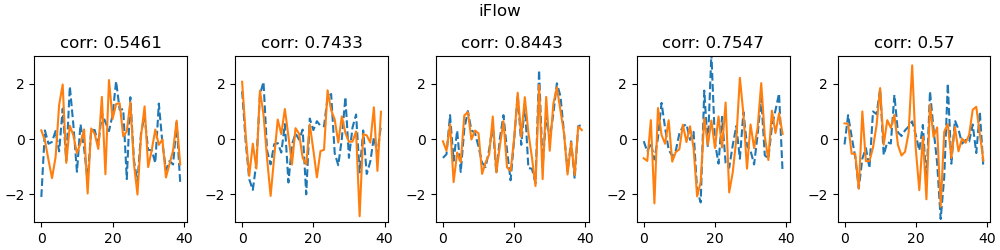
\includegraphics[width=0.8\textwidth]{Reproducibility_Challenge_2020/IMG/latent_corr/iFlow_92.png}
    \end{minipage}
    \begin{minipage}[b]{\textwidth}
    \centering
       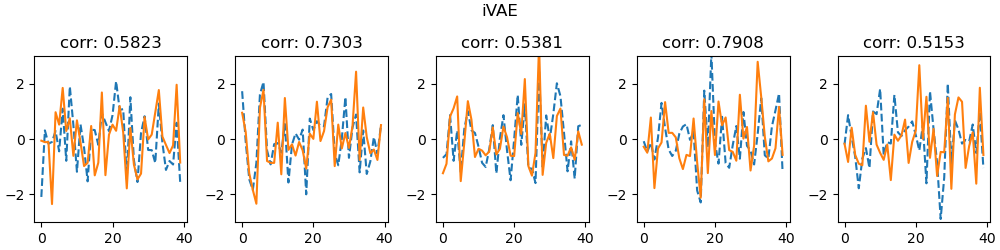
\includegraphics[width=0.8\textwidth]{Reproducibility_Challenge_2020/IMG/latent_corr/best_iVAE_92.png}
    \end{minipage}
    \caption{Comparison of the latent variables recovered by the models (orange lines) to the true latent variables (dashed blue lines) for individual dimensions. This figure shows results for the seed that resulted in the best iVAE performance.}
    \label{fig:latentcorr2}
\end{figure}

\newpage

\subsection{Results beyond original paper}
%============================ DESCRIPTION ================================
% Often papers don't include enough information to fully specify their experiments, so some additional experimentation may be necessary. For example, it might be the case that batch size was not specified, and so different batch sizes need to be evaluated to reproduce the original results. Include the results of any additional experiments here. Note: this won't be necessary for all reproductions.
%============================ CONTENT ================================

\subsubsection{Improved baseline}
\label{sec:alt methods}
In figure \ref{fig:MCCscores_Fixed:a} and \ref{fig:MCCscores_Fixed:b} the MCC scores and energy values over 100 seeds are displayed for the iFlow model, iVAE model and improved iVAE model. The addition of the trainable mean, based on auxiliary parameters, shows an increase in the mean MCC score from 0.483 (0.059) to 0.556 (0.061). The ELBO score improves almost with a constant value for every seed.

Other attempts had been made to improve this baseline by increasing the complexity of the iVAE model. However, were tried before the mistake in the iVAE implementation had been noticed, and are therefore not very useful. These results can be seen in appendix \ref{sec:baselineexperiments}.

In addition to figure \ref{fig:MCCscores}, recreations of figures \ref{fig:2D} \ref{fig:latentcorr1} using the improved baseline were made. These are not included in this report but can be found in appendix \ref{sec:appendixC}

\begin{figure}[htb]
  \begin{subfigure}[b]{0.5\textwidth}
    \centering
    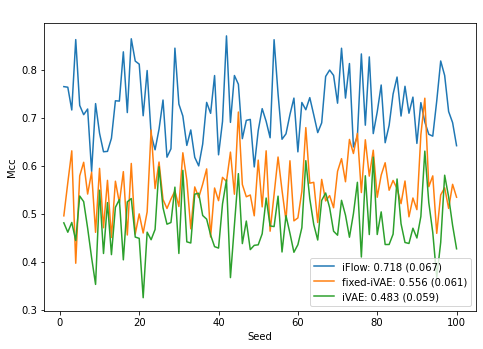
\includegraphics[width=\textwidth]{Reproducibility_Challenge_2020/IMG/scores/Mcc_Score_fixed.png}
    \caption{}
    \label{fig:MCCscores_Fixed:a}
  \end{subfigure}%%
  \begin{subfigure}[b]{0.5\textwidth}
    \centering
    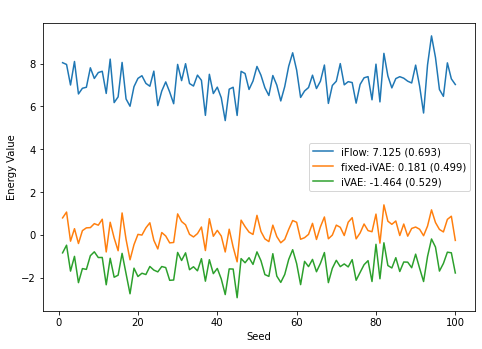
\includegraphics[width=\textwidth]{Reproducibility_Challenge_2020/IMG/scores/Log_Likelihood_fixed.png}
    \caption{}
    \label{fig:MCCscores_Fixed:b}
  \end{subfigure}
  \caption{Comparison of identifying performance (MCC) and the energy value (log-likelihood) versus seed number respectively, with the fixed version iVAE included.}
  \label{fig:MCCscores_Fixed}
\end{figure}

\subsubsection{Synthetic data complexity}
To measure the complexity of the dataset, the mean Kullback-Leibler divergence \cite{kullback1951information} of each source and its nearest neighbour was used.

This metric showed no correlation (0.06) with the MCC scores obtained by iVAE or iFlow, showing that the randomly sampled parameters of the source distribution were likely not to blame for the high variance in MCC scores.

\section{Discussion}
%============================ DESCRIPTION ================================
% Give your judgement on if your experimental results support the claims of the paper. Discuss the strengths and weaknesses of your approach - perhaps you didn't have time to run all the experiments, or perhaps you did additional experiments that further strengthened the claims in the paper.
%============================ CONTENT================================
The results reproduced in the previous section largely support the claims by the original authors. Firstly, the MCC scores that we obtained after training the model on synthetic data are very similar to the ones reported. Secondly, the recreated visualisation of 2D latent sources seems to support the claim that the iFlow method outperforms iVAE in identifying the original sources. Finally, the claim that iFlow exhibits much stronger correlation than iVAE in each single dimension of the latent space is not fully supported by our results. In the original paper, the authors show this correlation only for the best iFlow results. When visualising the individual dimensions of the latent variables for the best iVAE results, iVAE outperforms iFlow in two of the latent dimensions. This shows that the claim does not strictly hold true for all seeds. Nevertheless, since iFlow outperforms even the best iVAE on most latent dimensions, it still seems to be a reasonable claim.

Our experiments to improve the performance of the iVAE model, by modelling the prior means as a trainable function of the auxiliary variable $u$, managed to increase its performance significantly. However, the performance remains worse than that of iFlow. This further cements the claim that the iFlow model is more suited for the task of identifiability than iVAE.

% STRENGTHS
The strength of our approach was that we were generally faithful to the original implementation, using largely the same code which we examined thoroughly. Therefore, the chance of implementation differences with the original code is very small. Additionally, we rigorously compared the code with the underlying theory, allowing us to correct an important mistake in the baseline.

% WEAKNESSES
A weakness of our approach was that we did not do any work to examine the models on a more realistic dataset, meaning the generalisability of the model remains an open question. Furthermore, due to the high variance in the results of identifying models, all experiments had to be run with a large number of seeds (100), which took a long time given the fact that training of a single model took approximately 40 minutes. For this reason, experimentation done with hyperparameters was limited. The experiments in the appendix of the paper were not replicated for similar reasons. These experiments looked at the effect of different activation functions on the performance of iFlow and the effect of more and larger hidden layers on the performance of iVAE.
% Strengths and weaknesses of our research \\
% Strengths
%     \begin{enumerate}
%         \item Tested alternative version of iFlow with Softplus exerted only on $\xi$
%         \item Tested additional VAE models / improved iVAE performance for more fair comparison
%         \item Found improved baseline
%     \end{enumerate}
% Weakness
%     \begin{enumerate}
%         \item Less focus on theoretical background
%         \item Did not verify Appendix A1
%         \item maybe not enough hyperparameters search (for 2D)
%     \end{enumerate}

Overall, the authors provided a model which outperforms the previously best method for this problem in a quantifiable measure. Additionally, high variance in the results is addressed appropriately by running the experiments over a large number of seeds. Furthermore, the visualisation of the true sources and the estimations by the models makes it easier to interpret the MCC scores. Lastly, the model is theoretically well motivated.

Despite these strengths of the original paper, some improvements could be made to further substantiate the claims made in the paper.
There is a clear advantage that iVAE has over iFlow, which is not mentioned by the authors: iVAE can be used when the dimensionality of the latent sources differs from the data dimensionality, while iFlow cannot. The fact that iFlow needs data with such corresponding dimensionalities also means that the iVAE had to be trained without a bottleneck. This is an important part of the VAE architecture, and the lack thereof could have contributed to the weaker performance of iVAE; compared to the paper introducing iVAE (MCC of above 0.95), the MCC scores of the iVAE reported by the authors are significantly worse (MCC of 0.496). This discrepancy is not addressed or explained by the authors.

% Furthermore, the decrease in performance of the iVAE compared to the original iVAE paper were not addressed or explained. The original iVAE paper reported an MCC score of above 0.95 using the same dataset while an MCC score of 0.496 was achieved in this paper.

%
% Strengths and weaknesses of iFlow Paper \\
% Strengths
%     \begin{enumerate}
%         \item Strong theoretical background (Can we say this when we have not verified the background?)
%         \item iFlow outperforms iVAE
%         \item nice visualization
%         \item Many seeds are run
%     \end{enumerate}
% Weakness
%     \begin{enumerate}
%         \item Poor performance of iVAE compared to original paper not explained
%         \item Imprecise and careless documentation of experimental setup (Dataset, hyperparameters etc.)
%         \item Figure 3 cherry picked
%         \item Weak analysis of results
%         \item comparing model of $\sim 3M$ params  vs $\sim 18K$ (Somewhat justified in appendix)
%         \item maybe: code runs very inefficient
%         \item Baseline is a iVAE without bottleneck, which is crucial for a VAE to function well
%         \item The fact that the iFlow model cannot handle latent variables of different dimensionality than the data is not mentioned.
%     \end{enumerate}

\subsection{What was easy}
%============================ DESCRIPTION ================================
% Give your judgement of what was easy to reproduce. Perhaps the author's code is clearly written and easy to run, so it was easy to verify the majority of original claims. Or, the explanation in the paper was really easy to follow and put into code.
% Be careful not to give sweeping generalisations. Something that is easy for you might be difficult to others. Put what was easy in context and explain why it was easy (e.g. code had extensive API documentation and a lot of examples that matched experiments in papers).
%============================ CONTENT ================================
The code provided in the GitHub repository worked almost out of the box, with only small adjustments needed; the source code of the nflows library that was included in the repository was replaced with an import. This fixed an issue that prevented the code from running on a CPU.
The code was well organised into separate files for e.g., the iFlow model, iVAE models or training, making it easy to quickly find specific parts of the code when needed. The code that generates the data the models are trained on also came with the implementation, and worked without any issues.

With the code, a shell script was provided that seems to be the one used for the experiments on iFlow in the paper (although this was not explicitly stated). This allowed for easy replication of these experiments, with all of the used hyperparameters provided.

\subsection{What was difficult}
%============================ DESCRIPTION ================================
% List part of the reproduction study that took more time than you anticipated or you felt were difficult.
% Be careful to put your discussion in context. For example, don't say "the maths was difficult to follow", say "the math requires advanced knowledge of calculus to follow".
%============================ CONTENT ================================

There were difficulties in replicating some parts of the paper. The lack of a provided environment means that our code was likely run using different versions of some libraries such as PyTorch or NumPy. This could have contributed to the difference in outcomes of our experiments compared to the paper while using the same seeds.

While the script used to run iFlow experiments was provided, the same was not true for the iVAE experiments. This was not a large problem, however, since the authors do state that the hyperparameters used are the same as in the original iVAE paper \cite{khemakhem2020variational}. The code for creating plots (Figures 1,2,3 in the iFlow paper) was also not provided and additional code had to be written to recreate these figures.

The training of the iFlow models for all 100 seeds took a significant amount of time. With the training for one seed taking approximately 40 minutes, the full training took roughly a day and a half (running two batches of 50 seeds simultaneously). This made it difficult to do full-scale experiments with different hyperparameters.

Lastly, there was a large portion of unused code present in the repository, which made it more difficult to understand the overall structure of the code. This includes the source code of the nflows library, code for planar flows, multiple different iVAE variations, an alternative dataloader, an unused dataset and an implementation of training using annealing.

% \subsection{Communication with original authors}
% %============================ DESCRIPTION ================================
% % Document the extent of (or lack of) communication with the original authors. To make sure the reproducibility report is a fair assessment of the original research we recommend getting in touch with the original authors. You can ask authors specific questions, or if you don't have any questions you can send them the full report to get their feedback before it gets published.
% %  ========================== CONTENT ===================================

% Attempts at communication with the original author of the paper did not succeed. An email was sent to the author requesting additional information about software versions and some clarifications on the "simulations" section of the original paper. Unfortunately, we did not receive a reaction to these requests.
